\section{Database Design}
\label{sec:database_design}

The database schema is designed to support user account management, secure authentication, subscription tracking, and flexible service plan versioning. MongoDB's document-oriented approach provides the flexibility needed for an evolving application while maintaining data consistency and relationships.

\subsection{Core Data Model}

The system manages several interconnected data domains. The \textbf{Users} collection is the foundation, storing user account information including email, authentication credentials, user roles, and subscription status. Each user account can have an associated \textbf{Subscription}, which tracks their current service plan, usage quotas, and billing integration with external payment systems. The \textbf{Plans} collection maintains versioned service offerings, allowing the business to introduce new plans or modify existing ones without disrupting active subscriptions.

To support secure session management, two additional collections manage authentication state. The \textbf{UserTokens} collection tracks active authentication tokens for each user session, storing metadata such as token expiration time and client information. The \textbf{TokenBlacklist} collection maintains a record of revoked tokens, ensuring that logged-out users or users with invalidated sessions cannot reuse their old authentication credentials. Both collections leverage MongoDB's automatic expiration (TTL) feature to clean up old entries without manual intervention.

\subsection{Entity Relationships}

Figure~\ref{fig:er_diagram} illustrates how these collections relate to one another:

\begin{figure}[H]
\centering
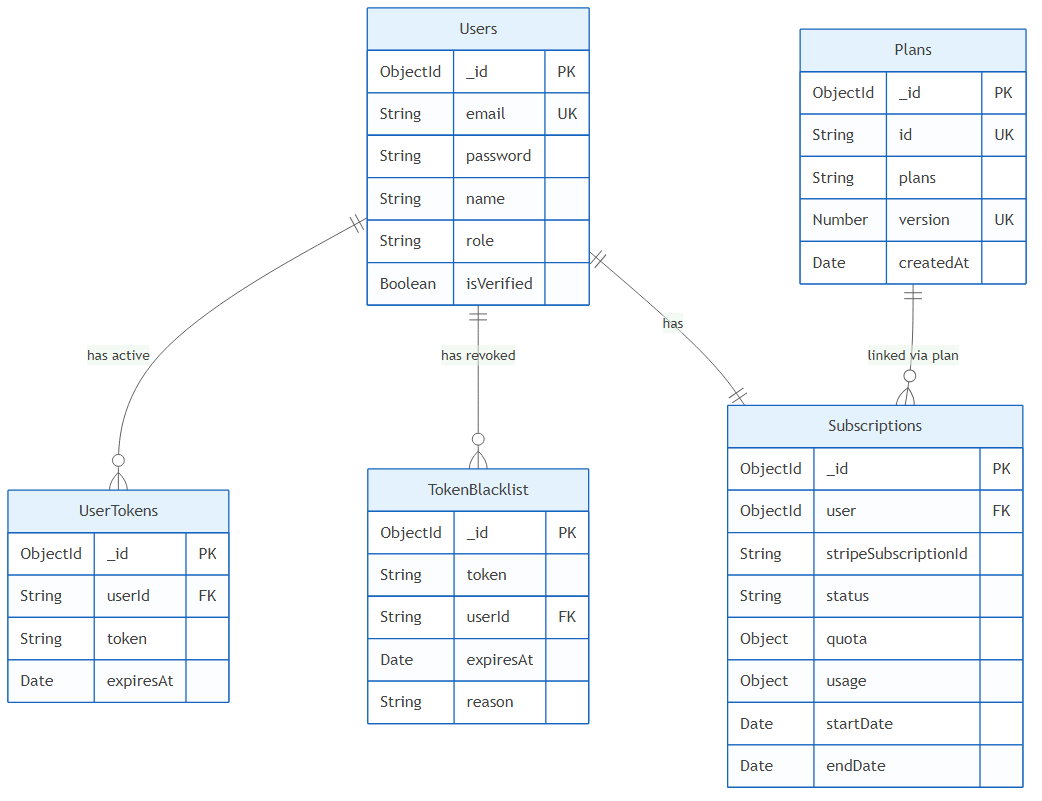
\includegraphics[width=0.75\textwidth]{images/er_diagram.png}
\caption{Entity Relationship Diagram}
\label{fig:er_diagram}
\end{figure}

The data model reflects common business logic. Each user maintains at most one active subscription, creating a one-to-one relationship. A subscription references an available plan and integrates with Stripe to track billing information. Users may have multiple active authentication tokens (for different devices or sessions), creating a one-to-many relationship. When users log out or sessions are invalidated, their tokens are moved to the blacklist to prevent reuse. The Plans collection exists independently but is logically referenced by subscriptions, enabling the application to manage plan availability and pricing changes without affecting existing customer data.

\subsection{Design Decisions}

The database schema reflects several key design principles. By storing user account information, subscription details, and authentication tokens in separate collections, the schema maintains clean separation of concerns—account data, billing data, and session management can be queried and updated independently. The use of document-based storage allows subscription records to embed service quota and usage information, making it efficient to retrieve complete subscription details in a single database operation. Token expiration handling through TTL indexes eliminates the need for periodic cleanup jobs, reducing operational complexity. This design balances normalization (separating logically distinct concepts) with denormalization (embedding related data to minimize joins), a practical approach for document databases like MongoDB.
